\documentclass[twoside]{book}

% Packages required by doxygen
\usepackage{calc}
\usepackage{doxygen}
\usepackage{graphicx}
\usepackage[utf8]{inputenc}
\usepackage{makeidx}
\usepackage{multicol}
\usepackage{multirow}
\usepackage{textcomp}
\usepackage[table]{xcolor}

% Font selection
\usepackage[T1]{fontenc}
\usepackage{mathptmx}
\usepackage[scaled=.90]{helvet}
\usepackage{courier}
\usepackage{amssymb}
\usepackage{sectsty}
\renewcommand{\familydefault}{\sfdefault}
\allsectionsfont{%
  \fontseries{bc}\selectfont%
  \color{darkgray}%
}
\renewcommand{\DoxyLabelFont}{%
  \fontseries{bc}\selectfont%
  \color{darkgray}%
}

% Page & text layout
\usepackage{geometry}
\geometry{%
  a4paper,%
  top=2.5cm,%
  bottom=2.5cm,%
  left=2.5cm,%
  right=2.5cm%
}
\tolerance=750
\hfuzz=15pt
\hbadness=750
\setlength{\emergencystretch}{15pt}
\setlength{\parindent}{0cm}
\setlength{\parskip}{0.2cm}
\makeatletter
\renewcommand{\paragraph}{%
  \@startsection{paragraph}{4}{0ex}{-1.0ex}{1.0ex}{%
    \normalfont\normalsize\bfseries\SS@parafont%
  }%
}
\renewcommand{\subparagraph}{%
  \@startsection{subparagraph}{5}{0ex}{-1.0ex}{1.0ex}{%
    \normalfont\normalsize\bfseries\SS@subparafont%
  }%
}
\makeatother

% Headers & footers
\usepackage{fancyhdr}
\pagestyle{fancyplain}
\fancyhead[LE]{\fancyplain{}{\bfseries\thepage}}
\fancyhead[CE]{\fancyplain{}{}}
\fancyhead[RE]{\fancyplain{}{\bfseries\leftmark}}
\fancyhead[LO]{\fancyplain{}{\bfseries\rightmark}}
\fancyhead[CO]{\fancyplain{}{}}
\fancyhead[RO]{\fancyplain{}{\bfseries\thepage}}
\fancyfoot[LE]{\fancyplain{}{}}
\fancyfoot[CE]{\fancyplain{}{}}
\fancyfoot[RE]{\fancyplain{}{\bfseries\scriptsize Generated on Wed Jan 8 2014 20\-:04\-:16 for Blinde Kuh by Doxygen }}
\fancyfoot[LO]{\fancyplain{}{\bfseries\scriptsize Generated on Wed Jan 8 2014 20\-:04\-:16 for Blinde Kuh by Doxygen }}
\fancyfoot[CO]{\fancyplain{}{}}
\fancyfoot[RO]{\fancyplain{}{}}
\renewcommand{\footrulewidth}{0.4pt}
\renewcommand{\chaptermark}[1]{%
  \markboth{#1}{}%
}
\renewcommand{\sectionmark}[1]{%
  \markright{\thesection\ #1}%
}

% Indices & bibliography
\usepackage{natbib}
\usepackage[titles]{tocloft}
\setcounter{tocdepth}{3}
\setcounter{secnumdepth}{5}
\makeindex

% Hyperlinks (required, but should be loaded last)
\usepackage{ifpdf}
\ifpdf
  \usepackage[pdftex,pagebackref=true]{hyperref}
\else
  \usepackage[ps2pdf,pagebackref=true]{hyperref}
\fi
\hypersetup{%
  colorlinks=true,%
  linkcolor=blue,%
  citecolor=blue,%
  unicode%
}

% Custom commands
\newcommand{\clearemptydoublepage}{%
  \newpage{\pagestyle{empty}\cleardoublepage}%
}


%===== C O N T E N T S =====

\begin{document}

% Titlepage & ToC
\hypersetup{pageanchor=false}
\pagenumbering{roman}
\begin{titlepage}
\vspace*{7cm}
\begin{center}%
{\Large Blinde Kuh \\[1ex]\large 1.\-0-\/\-S\-N\-A\-P\-S\-H\-O\-T }\\
\vspace*{1cm}
{\large Generated by Doxygen 1.8.5}\\
\vspace*{0.5cm}
{\small Wed Jan 8 2014 20:04:16}\\
\end{center}
\end{titlepage}
\clearemptydoublepage
\tableofcontents
\clearemptydoublepage
\pagenumbering{arabic}
\hypersetup{pageanchor=true}

%--- Begin generated contents ---
\chapter{bl\-Kuh}
\label{md__d_1_projects_bl_kuh__r_e_a_d_m_e}
\hypertarget{md__d_1_projects_bl_kuh__r_e_a_d_m_e}{}
Ein Blinde Kuh Spiel als Swing Applikation 
\chapter{Namespace Index}
\section{Packages}
Here are the packages with brief descriptions (if available)\-:\begin{DoxyCompactList}
\item\contentsline{section}{\hyperlink{namespacebl_kuh}{bl\-Kuh} }{\pageref{namespacebl_kuh}}{}
\item\contentsline{section}{\hyperlink{namespacede}{de} }{\pageref{namespacede}}{}
\item\contentsline{section}{\hyperlink{namespacede_1_1htw}{de.\-htw} }{\pageref{namespacede_1_1htw}}{}
\item\contentsline{section}{\hyperlink{namespacede_1_1htw_1_1berlin}{de.\-htw.\-berlin} }{\pageref{namespacede_1_1htw_1_1berlin}}{}
\item\contentsline{section}{\hyperlink{namespacede_1_1htw_1_1berlin_1_1student}{de.\-htw.\-berlin.\-student} }{\pageref{namespacede_1_1htw_1_1berlin_1_1student}}{}
\item\contentsline{section}{\hyperlink{namespacede_1_1htw_1_1berlin_1_1student_1_1bl_kuh}{de.\-htw.\-berlin.\-student.\-bl\-Kuh} }{\pageref{namespacede_1_1htw_1_1berlin_1_1student_1_1bl_kuh}}{}
\item\contentsline{section}{\hyperlink{namespacede_1_1htw_1_1berlin_1_1student_1_1bl_kuh_1_1component}{de.\-htw.\-berlin.\-student.\-bl\-Kuh.\-component} }{\pageref{namespacede_1_1htw_1_1berlin_1_1student_1_1bl_kuh_1_1component}}{}
\item\contentsline{section}{\hyperlink{namespacede_1_1htw_1_1berlin_1_1student_1_1bl_kuh_1_1exceptions}{de.\-htw.\-berlin.\-student.\-bl\-Kuh.\-exceptions} }{\pageref{namespacede_1_1htw_1_1berlin_1_1student_1_1bl_kuh_1_1exceptions}}{}
\item\contentsline{section}{\hyperlink{namespacede_1_1htw_1_1berlin_1_1student_1_1bl_kuh_1_1menu}{de.\-htw.\-berlin.\-student.\-bl\-Kuh.\-menu} }{\pageref{namespacede_1_1htw_1_1berlin_1_1student_1_1bl_kuh_1_1menu}}{}
\item\contentsline{section}{\hyperlink{namespacede_1_1htw_1_1berlin_1_1student_1_1bl_kuh_1_1model}{de.\-htw.\-berlin.\-student.\-bl\-Kuh.\-model} }{\pageref{namespacede_1_1htw_1_1berlin_1_1student_1_1bl_kuh_1_1model}}{}
\item\contentsline{section}{\hyperlink{namespacede_1_1htw_1_1berlin_1_1student_1_1bl_kuh_1_1view}{de.\-htw.\-berlin.\-student.\-bl\-Kuh.\-view} }{\pageref{namespacede_1_1htw_1_1berlin_1_1student_1_1bl_kuh_1_1view}}{}
\end{DoxyCompactList}

\chapter{Hierarchical Index}
\section{Class Hierarchy}
This inheritance list is sorted roughly, but not completely, alphabetically\-:\begin{DoxyCompactList}
\item Exception\begin{DoxyCompactList}
\item \contentsline{section}{de.\-htw.\-berlin.\-student.\-bl\-Kuh.\-exceptions.\-No\-Neighbors\-Exception}{\pageref{classde_1_1htw_1_1berlin_1_1student_1_1bl_kuh_1_1exceptions_1_1_no_neighbors_exception}}{}
\end{DoxyCompactList}
\item \contentsline{section}{de.\-htw.\-berlin.\-student.\-bl\-Kuh.\-Main}{\pageref{classde_1_1htw_1_1berlin_1_1student_1_1bl_kuh_1_1_main}}{}
\item \contentsline{section}{de.\-htw.\-berlin.\-student.\-bl\-Kuh.\-menu.\-Menu\-Items}{\pageref{enumde_1_1htw_1_1berlin_1_1student_1_1bl_kuh_1_1menu_1_1_menu_items}}{}
\item \contentsline{section}{bl\-Kuh.\-Randomizer\-Test}{\pageref{classbl_kuh_1_1_randomizer_test}}{}
\item \contentsline{section}{de.\-htw.\-berlin.\-student.\-bl\-Kuh.\-model.\-Settings}{\pageref{classde_1_1htw_1_1berlin_1_1student_1_1bl_kuh_1_1model_1_1_settings}}{}
\item \contentsline{section}{de.\-htw.\-berlin.\-student.\-bl\-Kuh.\-Spielfeld}{\pageref{classde_1_1htw_1_1berlin_1_1student_1_1bl_kuh_1_1_spielfeld}}{}
\item Action\-Listener\begin{DoxyCompactList}
\item \contentsline{section}{de.\-htw.\-berlin.\-student.\-bl\-Kuh.\-Main\-Window}{\pageref{classde_1_1htw_1_1berlin_1_1student_1_1bl_kuh_1_1_main_window}}{}
\end{DoxyCompactList}
\item J\-Button\begin{DoxyCompactList}
\item \contentsline{section}{de.\-htw.\-berlin.\-student.\-bl\-Kuh.\-component.\-Tile\-Button}{\pageref{classde_1_1htw_1_1berlin_1_1student_1_1bl_kuh_1_1component_1_1_tile_button}}{}
\end{DoxyCompactList}
\item J\-Frame\begin{DoxyCompactList}
\item \contentsline{section}{de.\-htw.\-berlin.\-student.\-bl\-Kuh.\-Main\-Window}{\pageref{classde_1_1htw_1_1berlin_1_1student_1_1bl_kuh_1_1_main_window}}{}
\end{DoxyCompactList}
\item J\-Panel\begin{DoxyCompactList}
\item \contentsline{section}{de.\-htw.\-berlin.\-student.\-bl\-Kuh.\-view.\-Options\-View}{\pageref{classde_1_1htw_1_1berlin_1_1student_1_1bl_kuh_1_1view_1_1_options_view}}{}
\item \contentsline{section}{de.\-htw.\-berlin.\-student.\-bl\-Kuh.\-view.\-Spielfeld\-View}{\pageref{classde_1_1htw_1_1berlin_1_1student_1_1bl_kuh_1_1view_1_1_spielfeld_view}}{}
\end{DoxyCompactList}
\end{DoxyCompactList}

\chapter{Class Index}
\section{Class List}
Here are the classes, structs, unions and interfaces with brief descriptions\-:\begin{DoxyCompactList}
\item\contentsline{section}{\hyperlink{classde_1_1htw_1_1berlin_1_1student_1_1bl_kuh_1_1_main}{de.\-htw.\-berlin.\-student.\-bl\-Kuh.\-Main} }{\pageref{classde_1_1htw_1_1berlin_1_1student_1_1bl_kuh_1_1_main}}{}
\item\contentsline{section}{\hyperlink{classde_1_1htw_1_1berlin_1_1student_1_1bl_kuh_1_1_main_window}{de.\-htw.\-berlin.\-student.\-bl\-Kuh.\-Main\-Window} }{\pageref{classde_1_1htw_1_1berlin_1_1student_1_1bl_kuh_1_1_main_window}}{}
\item\contentsline{section}{\hyperlink{enumde_1_1htw_1_1berlin_1_1student_1_1bl_kuh_1_1menu_1_1_menu_items}{de.\-htw.\-berlin.\-student.\-bl\-Kuh.\-menu.\-Menu\-Items} }{\pageref{enumde_1_1htw_1_1berlin_1_1student_1_1bl_kuh_1_1menu_1_1_menu_items}}{}
\item\contentsline{section}{\hyperlink{classde_1_1htw_1_1berlin_1_1student_1_1bl_kuh_1_1exceptions_1_1_no_neighbors_exception}{de.\-htw.\-berlin.\-student.\-bl\-Kuh.\-exceptions.\-No\-Neighbors\-Exception} }{\pageref{classde_1_1htw_1_1berlin_1_1student_1_1bl_kuh_1_1exceptions_1_1_no_neighbors_exception}}{}
\item\contentsline{section}{\hyperlink{classde_1_1htw_1_1berlin_1_1student_1_1bl_kuh_1_1view_1_1_options_view}{de.\-htw.\-berlin.\-student.\-bl\-Kuh.\-view.\-Options\-View} }{\pageref{classde_1_1htw_1_1berlin_1_1student_1_1bl_kuh_1_1view_1_1_options_view}}{}
\item\contentsline{section}{\hyperlink{classbl_kuh_1_1_randomizer_test}{bl\-Kuh.\-Randomizer\-Test} }{\pageref{classbl_kuh_1_1_randomizer_test}}{}
\item\contentsline{section}{\hyperlink{classde_1_1htw_1_1berlin_1_1student_1_1bl_kuh_1_1model_1_1_settings}{de.\-htw.\-berlin.\-student.\-bl\-Kuh.\-model.\-Settings} }{\pageref{classde_1_1htw_1_1berlin_1_1student_1_1bl_kuh_1_1model_1_1_settings}}{}
\item\contentsline{section}{\hyperlink{classde_1_1htw_1_1berlin_1_1student_1_1bl_kuh_1_1_spielfeld}{de.\-htw.\-berlin.\-student.\-bl\-Kuh.\-Spielfeld} }{\pageref{classde_1_1htw_1_1berlin_1_1student_1_1bl_kuh_1_1_spielfeld}}{}
\item\contentsline{section}{\hyperlink{classde_1_1htw_1_1berlin_1_1student_1_1bl_kuh_1_1view_1_1_spielfeld_view}{de.\-htw.\-berlin.\-student.\-bl\-Kuh.\-view.\-Spielfeld\-View} }{\pageref{classde_1_1htw_1_1berlin_1_1student_1_1bl_kuh_1_1view_1_1_spielfeld_view}}{}
\item\contentsline{section}{\hyperlink{classde_1_1htw_1_1berlin_1_1student_1_1bl_kuh_1_1component_1_1_tile_button}{de.\-htw.\-berlin.\-student.\-bl\-Kuh.\-component.\-Tile\-Button} }{\pageref{classde_1_1htw_1_1berlin_1_1student_1_1bl_kuh_1_1component_1_1_tile_button}}{}
\end{DoxyCompactList}

\chapter{File Index}
\section{File List}
Here is a list of all files with brief descriptions\-:\begin{DoxyCompactList}
\item\contentsline{section}{D\-:/projects/bl\-Kuh/src/main/java/de/htw/berlin/student/bl\-Kuh/\hyperlink{_main_8java}{Main.\-java} }{\pageref{_main_8java}}{}
\item\contentsline{section}{D\-:/projects/bl\-Kuh/src/main/java/de/htw/berlin/student/bl\-Kuh/\hyperlink{_main_window_8java}{Main\-Window.\-java} }{\pageref{_main_window_8java}}{}
\item\contentsline{section}{D\-:/projects/bl\-Kuh/src/main/java/de/htw/berlin/student/bl\-Kuh/\hyperlink{_spielfeld_8java}{Spielfeld.\-java} }{\pageref{_spielfeld_8java}}{}
\item\contentsline{section}{D\-:/projects/bl\-Kuh/src/main/java/de/htw/berlin/student/bl\-Kuh/component/\hyperlink{_tile_button_8java}{Tile\-Button.\-java} }{\pageref{_tile_button_8java}}{}
\item\contentsline{section}{D\-:/projects/bl\-Kuh/src/main/java/de/htw/berlin/student/bl\-Kuh/exceptions/\hyperlink{_no_neighbors_exception_8java}{No\-Neighbors\-Exception.\-java} }{\pageref{_no_neighbors_exception_8java}}{}
\item\contentsline{section}{D\-:/projects/bl\-Kuh/src/main/java/de/htw/berlin/student/bl\-Kuh/menu/\hyperlink{_menu_items_8java}{Menu\-Items.\-java} }{\pageref{_menu_items_8java}}{}
\item\contentsline{section}{D\-:/projects/bl\-Kuh/src/main/java/de/htw/berlin/student/bl\-Kuh/model/\hyperlink{_settings_8java}{Settings.\-java} }{\pageref{_settings_8java}}{}
\item\contentsline{section}{D\-:/projects/bl\-Kuh/src/main/java/de/htw/berlin/student/bl\-Kuh/view/\hyperlink{_options_view_8java}{Options\-View.\-java} }{\pageref{_options_view_8java}}{}
\item\contentsline{section}{D\-:/projects/bl\-Kuh/src/main/java/de/htw/berlin/student/bl\-Kuh/view/\hyperlink{_spielfeld_view_8java}{Spielfeld\-View.\-java} }{\pageref{_spielfeld_view_8java}}{}
\item\contentsline{section}{D\-:/projects/bl\-Kuh/src/test/java/bl\-Kuh/\hyperlink{_randomizer_test_8java}{Randomizer\-Test.\-java} }{\pageref{_randomizer_test_8java}}{}
\end{DoxyCompactList}

\chapter{Namespace Documentation}
\hypertarget{namespacebl_kuh}{\section{Package bl\-Kuh}
\label{namespacebl_kuh}\index{bl\-Kuh@{bl\-Kuh}}
}
\subsection*{Classes}
\begin{DoxyCompactItemize}
\item 
class \hyperlink{classbl_kuh_1_1_randomizer_test}{Randomizer\-Test}
\end{DoxyCompactItemize}

\hypertarget{namespacede}{\section{Package de}
\label{namespacede}\index{de@{de}}
}
\subsection*{Packages}
\begin{DoxyCompactItemize}
\item 
package \hyperlink{namespacede_1_1htw}{htw}
\end{DoxyCompactItemize}

\hypertarget{namespacede_1_1htw}{\section{Package de.\-htw}
\label{namespacede_1_1htw}\index{de.\-htw@{de.\-htw}}
}
\subsection*{Packages}
\begin{DoxyCompactItemize}
\item 
package \hyperlink{namespacede_1_1htw_1_1berlin}{berlin}
\end{DoxyCompactItemize}

\hypertarget{namespacede_1_1htw_1_1berlin}{\section{Package de.\-htw.\-berlin}
\label{namespacede_1_1htw_1_1berlin}\index{de.\-htw.\-berlin@{de.\-htw.\-berlin}}
}
\subsection*{Packages}
\begin{DoxyCompactItemize}
\item 
package \hyperlink{namespacede_1_1htw_1_1berlin_1_1student}{student}
\end{DoxyCompactItemize}

\hypertarget{namespacede_1_1htw_1_1berlin_1_1student}{\section{Package de.\-htw.\-berlin.\-student}
\label{namespacede_1_1htw_1_1berlin_1_1student}\index{de.\-htw.\-berlin.\-student@{de.\-htw.\-berlin.\-student}}
}
\subsection*{Packages}
\begin{DoxyCompactItemize}
\item 
package \hyperlink{namespacede_1_1htw_1_1berlin_1_1student_1_1bl_kuh}{bl\-Kuh}
\end{DoxyCompactItemize}

\hypertarget{namespacede_1_1htw_1_1berlin_1_1student_1_1bl_kuh}{\section{Package de.\-htw.\-berlin.\-student.\-bl\-Kuh}
\label{namespacede_1_1htw_1_1berlin_1_1student_1_1bl_kuh}\index{de.\-htw.\-berlin.\-student.\-bl\-Kuh@{de.\-htw.\-berlin.\-student.\-bl\-Kuh}}
}
\subsection*{Packages}
\begin{DoxyCompactItemize}
\item 
package \hyperlink{namespacede_1_1htw_1_1berlin_1_1student_1_1bl_kuh_1_1component}{component}
\item 
package \hyperlink{namespacede_1_1htw_1_1berlin_1_1student_1_1bl_kuh_1_1exceptions}{exceptions}
\item 
package \hyperlink{namespacede_1_1htw_1_1berlin_1_1student_1_1bl_kuh_1_1menu}{menu}
\item 
package \hyperlink{namespacede_1_1htw_1_1berlin_1_1student_1_1bl_kuh_1_1model}{model}
\item 
package \hyperlink{namespacede_1_1htw_1_1berlin_1_1student_1_1bl_kuh_1_1view}{view}
\end{DoxyCompactItemize}
\subsection*{Classes}
\begin{DoxyCompactItemize}
\item 
class \hyperlink{classde_1_1htw_1_1berlin_1_1student_1_1bl_kuh_1_1_main}{Main}
\item 
class \hyperlink{classde_1_1htw_1_1berlin_1_1student_1_1bl_kuh_1_1_main_window}{Main\-Window}
\item 
class \hyperlink{classde_1_1htw_1_1berlin_1_1student_1_1bl_kuh_1_1_spielfeld}{Spielfeld}
\end{DoxyCompactItemize}

\hypertarget{namespacede_1_1htw_1_1berlin_1_1student_1_1bl_kuh_1_1component}{\section{Package de.\-htw.\-berlin.\-student.\-bl\-Kuh.\-component}
\label{namespacede_1_1htw_1_1berlin_1_1student_1_1bl_kuh_1_1component}\index{de.\-htw.\-berlin.\-student.\-bl\-Kuh.\-component@{de.\-htw.\-berlin.\-student.\-bl\-Kuh.\-component}}
}
\subsection*{Classes}
\begin{DoxyCompactItemize}
\item 
class \hyperlink{classde_1_1htw_1_1berlin_1_1student_1_1bl_kuh_1_1component_1_1_tile_button}{Tile\-Button}
\end{DoxyCompactItemize}

\hypertarget{namespacede_1_1htw_1_1berlin_1_1student_1_1bl_kuh_1_1exceptions}{\section{Package de.\-htw.\-berlin.\-student.\-bl\-Kuh.\-exceptions}
\label{namespacede_1_1htw_1_1berlin_1_1student_1_1bl_kuh_1_1exceptions}\index{de.\-htw.\-berlin.\-student.\-bl\-Kuh.\-exceptions@{de.\-htw.\-berlin.\-student.\-bl\-Kuh.\-exceptions}}
}
\subsection*{Classes}
\begin{DoxyCompactItemize}
\item 
class \hyperlink{classde_1_1htw_1_1berlin_1_1student_1_1bl_kuh_1_1exceptions_1_1_no_neighbors_exception}{No\-Neighbors\-Exception}
\end{DoxyCompactItemize}

\hypertarget{namespacede_1_1htw_1_1berlin_1_1student_1_1bl_kuh_1_1menu}{\section{Package de.\-htw.\-berlin.\-student.\-bl\-Kuh.\-menu}
\label{namespacede_1_1htw_1_1berlin_1_1student_1_1bl_kuh_1_1menu}\index{de.\-htw.\-berlin.\-student.\-bl\-Kuh.\-menu@{de.\-htw.\-berlin.\-student.\-bl\-Kuh.\-menu}}
}
\subsection*{Classes}
\begin{DoxyCompactItemize}
\item 
enum \hyperlink{enumde_1_1htw_1_1berlin_1_1student_1_1bl_kuh_1_1menu_1_1_menu_items}{Menu\-Items}
\end{DoxyCompactItemize}

\hypertarget{namespacede_1_1htw_1_1berlin_1_1student_1_1bl_kuh_1_1model}{\section{Package de.\-htw.\-berlin.\-student.\-bl\-Kuh.\-model}
\label{namespacede_1_1htw_1_1berlin_1_1student_1_1bl_kuh_1_1model}\index{de.\-htw.\-berlin.\-student.\-bl\-Kuh.\-model@{de.\-htw.\-berlin.\-student.\-bl\-Kuh.\-model}}
}
\subsection*{Classes}
\begin{DoxyCompactItemize}
\item 
class \hyperlink{classde_1_1htw_1_1berlin_1_1student_1_1bl_kuh_1_1model_1_1_settings}{Settings}
\end{DoxyCompactItemize}

\hypertarget{namespacede_1_1htw_1_1berlin_1_1student_1_1bl_kuh_1_1view}{\section{Package de.\-htw.\-berlin.\-student.\-bl\-Kuh.\-view}
\label{namespacede_1_1htw_1_1berlin_1_1student_1_1bl_kuh_1_1view}\index{de.\-htw.\-berlin.\-student.\-bl\-Kuh.\-view@{de.\-htw.\-berlin.\-student.\-bl\-Kuh.\-view}}
}
\subsection*{Classes}
\begin{DoxyCompactItemize}
\item 
class \hyperlink{classde_1_1htw_1_1berlin_1_1student_1_1bl_kuh_1_1view_1_1_options_view}{Options\-View}
\item 
class \hyperlink{classde_1_1htw_1_1berlin_1_1student_1_1bl_kuh_1_1view_1_1_spielfeld_view}{Spielfeld\-View}
\end{DoxyCompactItemize}

\chapter{Class Documentation}
\hypertarget{classde_1_1htw_1_1berlin_1_1student_1_1bl_kuh_1_1_main}{\section{de.\-htw.\-berlin.\-student.\-bl\-Kuh.\-Main Class Reference}
\label{classde_1_1htw_1_1berlin_1_1student_1_1bl_kuh_1_1_main}\index{de.\-htw.\-berlin.\-student.\-bl\-Kuh.\-Main@{de.\-htw.\-berlin.\-student.\-bl\-Kuh.\-Main}}
}
\subsection*{Static Public Member Functions}
\begin{DoxyCompactItemize}
\item 
static void \hyperlink{classde_1_1htw_1_1berlin_1_1student_1_1bl_kuh_1_1_main_a54a6320b6a93db61cb926b7bf2e54d53}{main} (String\mbox{[}$\,$\mbox{]} args)
\end{DoxyCompactItemize}


\subsection{Detailed Description}
\hyperlink{classde_1_1htw_1_1berlin_1_1student_1_1bl_kuh_1_1_main}{Main} class for the \hyperlink{namespacede_1_1htw_1_1berlin_1_1student_1_1bl_kuh}{bl\-Kuh} game.

\begin{DoxyAuthor}{Author}
Matthias Drummer 
\end{DoxyAuthor}


\subsection{Member Function Documentation}
\hypertarget{classde_1_1htw_1_1berlin_1_1student_1_1bl_kuh_1_1_main_a54a6320b6a93db61cb926b7bf2e54d53}{\index{de\-::htw\-::berlin\-::student\-::bl\-Kuh\-::\-Main@{de\-::htw\-::berlin\-::student\-::bl\-Kuh\-::\-Main}!main@{main}}
\index{main@{main}!de::htw::berlin::student::blKuh::Main@{de\-::htw\-::berlin\-::student\-::bl\-Kuh\-::\-Main}}
\subsubsection[{main}]{\setlength{\rightskip}{0pt plus 5cm}static void de.\-htw.\-berlin.\-student.\-bl\-Kuh.\-Main.\-main (
\begin{DoxyParamCaption}
\item[{String\mbox{[}$\,$\mbox{]}}]{args}
\end{DoxyParamCaption}
)\hspace{0.3cm}{\ttfamily [static]}}}\label{classde_1_1htw_1_1berlin_1_1student_1_1bl_kuh_1_1_main_a54a6320b6a93db61cb926b7bf2e54d53}


The documentation for this class was generated from the following file\-:\begin{DoxyCompactItemize}
\item 
D\-:/projects/bl\-Kuh/src/main/java/de/htw/berlin/student/bl\-Kuh/\hyperlink{_main_8java}{Main.\-java}\end{DoxyCompactItemize}

\hypertarget{classde_1_1htw_1_1berlin_1_1student_1_1bl_kuh_1_1_main_window}{\section{de.\-htw.\-berlin.\-student.\-bl\-Kuh.\-Main\-Window Class Reference}
\label{classde_1_1htw_1_1berlin_1_1student_1_1bl_kuh_1_1_main_window}\index{de.\-htw.\-berlin.\-student.\-bl\-Kuh.\-Main\-Window@{de.\-htw.\-berlin.\-student.\-bl\-Kuh.\-Main\-Window}}
}
Inheritance diagram for de.\-htw.\-berlin.\-student.\-bl\-Kuh.\-Main\-Window\-:\begin{figure}[H]
\begin{center}
\leavevmode
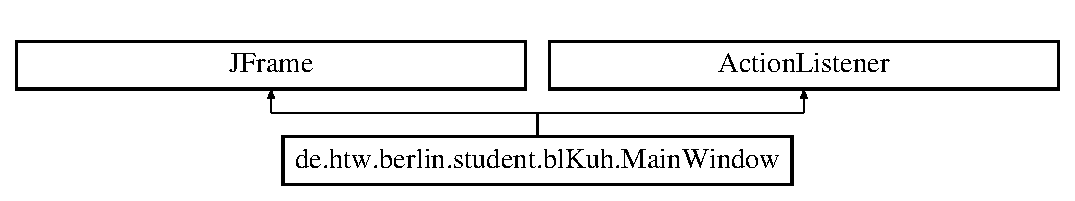
\includegraphics[height=2.000000cm]{classde_1_1htw_1_1berlin_1_1student_1_1bl_kuh_1_1_main_window}
\end{center}
\end{figure}
\subsection*{Public Member Functions}
\begin{DoxyCompactItemize}
\item 
\hyperlink{classde_1_1htw_1_1berlin_1_1student_1_1bl_kuh_1_1_main_window_af0fa47179b560817fe6c1da31fe4ed53}{Main\-Window} ()
\item 
void \hyperlink{classde_1_1htw_1_1berlin_1_1student_1_1bl_kuh_1_1_main_window_a5f1f3104069bf2aa0ba76471f7a70767}{action\-Performed} (Action\-Event e)
\end{DoxyCompactItemize}


\subsection{Detailed Description}
The main window of the \hyperlink{namespacede_1_1htw_1_1berlin_1_1student_1_1bl_kuh}{bl\-Kuh} swing application.

\begin{DoxyAuthor}{Author}
Matthias Drummer 

Marcel Piater 
\end{DoxyAuthor}


\subsection{Constructor \& Destructor Documentation}
\hypertarget{classde_1_1htw_1_1berlin_1_1student_1_1bl_kuh_1_1_main_window_af0fa47179b560817fe6c1da31fe4ed53}{\index{de\-::htw\-::berlin\-::student\-::bl\-Kuh\-::\-Main\-Window@{de\-::htw\-::berlin\-::student\-::bl\-Kuh\-::\-Main\-Window}!Main\-Window@{Main\-Window}}
\index{Main\-Window@{Main\-Window}!de::htw::berlin::student::blKuh::MainWindow@{de\-::htw\-::berlin\-::student\-::bl\-Kuh\-::\-Main\-Window}}
\subsubsection[{Main\-Window}]{\setlength{\rightskip}{0pt plus 5cm}de.\-htw.\-berlin.\-student.\-bl\-Kuh.\-Main\-Window.\-Main\-Window (
\begin{DoxyParamCaption}
{}
\end{DoxyParamCaption}
)}}\label{classde_1_1htw_1_1berlin_1_1student_1_1bl_kuh_1_1_main_window_af0fa47179b560817fe6c1da31fe4ed53}
Constructor. 

\subsection{Member Function Documentation}
\hypertarget{classde_1_1htw_1_1berlin_1_1student_1_1bl_kuh_1_1_main_window_a5f1f3104069bf2aa0ba76471f7a70767}{\index{de\-::htw\-::berlin\-::student\-::bl\-Kuh\-::\-Main\-Window@{de\-::htw\-::berlin\-::student\-::bl\-Kuh\-::\-Main\-Window}!action\-Performed@{action\-Performed}}
\index{action\-Performed@{action\-Performed}!de::htw::berlin::student::blKuh::MainWindow@{de\-::htw\-::berlin\-::student\-::bl\-Kuh\-::\-Main\-Window}}
\subsubsection[{action\-Performed}]{\setlength{\rightskip}{0pt plus 5cm}void de.\-htw.\-berlin.\-student.\-bl\-Kuh.\-Main\-Window.\-action\-Performed (
\begin{DoxyParamCaption}
\item[{Action\-Event}]{e}
\end{DoxyParamCaption}
)}}\label{classde_1_1htw_1_1berlin_1_1student_1_1bl_kuh_1_1_main_window_a5f1f3104069bf2aa0ba76471f7a70767}


The documentation for this class was generated from the following file\-:\begin{DoxyCompactItemize}
\item 
D\-:/projects/bl\-Kuh/src/main/java/de/htw/berlin/student/bl\-Kuh/\hyperlink{_main_window_8java}{Main\-Window.\-java}\end{DoxyCompactItemize}

\hypertarget{enumde_1_1htw_1_1berlin_1_1student_1_1bl_kuh_1_1menu_1_1_menu_items}{\section{de.\-htw.\-berlin.\-student.\-bl\-Kuh.\-menu.\-Menu\-Items Enum Reference}
\label{enumde_1_1htw_1_1berlin_1_1student_1_1bl_kuh_1_1menu_1_1_menu_items}\index{de.\-htw.\-berlin.\-student.\-bl\-Kuh.\-menu.\-Menu\-Items@{de.\-htw.\-berlin.\-student.\-bl\-Kuh.\-menu.\-Menu\-Items}}
}
\subsection*{Public Attributes}
\begin{DoxyCompactItemize}
\item 
\hyperlink{enumde_1_1htw_1_1berlin_1_1student_1_1bl_kuh_1_1menu_1_1_menu_items_a7b9c04ebd62b141b4c79c6520c4f1dc7}{N\-E\-W}
\item 
\hyperlink{enumde_1_1htw_1_1berlin_1_1student_1_1bl_kuh_1_1menu_1_1_menu_items_a91c5db842ee9aa831b0896a575e9909f}{E\-X\-I\-T}
\item 
\hyperlink{enumde_1_1htw_1_1berlin_1_1student_1_1bl_kuh_1_1menu_1_1_menu_items_aadca86423f12d3f0f457ff4d0aba01e2}{O\-P\-T\-I\-O\-N\-S}
\end{DoxyCompactItemize}


\subsection{Detailed Description}
Enum that provides possible menu items

\begin{DoxyAuthor}{Author}
Matthias Drummer 
\end{DoxyAuthor}


\subsection{Member Data Documentation}
\hypertarget{enumde_1_1htw_1_1berlin_1_1student_1_1bl_kuh_1_1menu_1_1_menu_items_a91c5db842ee9aa831b0896a575e9909f}{\index{de\-::htw\-::berlin\-::student\-::bl\-Kuh\-::menu\-::\-Menu\-Items@{de\-::htw\-::berlin\-::student\-::bl\-Kuh\-::menu\-::\-Menu\-Items}!E\-X\-I\-T@{E\-X\-I\-T}}
\index{E\-X\-I\-T@{E\-X\-I\-T}!de::htw::berlin::student::blKuh::menu::MenuItems@{de\-::htw\-::berlin\-::student\-::bl\-Kuh\-::menu\-::\-Menu\-Items}}
\subsubsection[{E\-X\-I\-T}]{\setlength{\rightskip}{0pt plus 5cm}de.\-htw.\-berlin.\-student.\-bl\-Kuh.\-menu.\-Menu\-Items.\-E\-X\-I\-T}}\label{enumde_1_1htw_1_1berlin_1_1student_1_1bl_kuh_1_1menu_1_1_menu_items_a91c5db842ee9aa831b0896a575e9909f}
\hypertarget{enumde_1_1htw_1_1berlin_1_1student_1_1bl_kuh_1_1menu_1_1_menu_items_a7b9c04ebd62b141b4c79c6520c4f1dc7}{\index{de\-::htw\-::berlin\-::student\-::bl\-Kuh\-::menu\-::\-Menu\-Items@{de\-::htw\-::berlin\-::student\-::bl\-Kuh\-::menu\-::\-Menu\-Items}!N\-E\-W@{N\-E\-W}}
\index{N\-E\-W@{N\-E\-W}!de::htw::berlin::student::blKuh::menu::MenuItems@{de\-::htw\-::berlin\-::student\-::bl\-Kuh\-::menu\-::\-Menu\-Items}}
\subsubsection[{N\-E\-W}]{\setlength{\rightskip}{0pt plus 5cm}de.\-htw.\-berlin.\-student.\-bl\-Kuh.\-menu.\-Menu\-Items.\-N\-E\-W}}\label{enumde_1_1htw_1_1berlin_1_1student_1_1bl_kuh_1_1menu_1_1_menu_items_a7b9c04ebd62b141b4c79c6520c4f1dc7}
\hypertarget{enumde_1_1htw_1_1berlin_1_1student_1_1bl_kuh_1_1menu_1_1_menu_items_aadca86423f12d3f0f457ff4d0aba01e2}{\index{de\-::htw\-::berlin\-::student\-::bl\-Kuh\-::menu\-::\-Menu\-Items@{de\-::htw\-::berlin\-::student\-::bl\-Kuh\-::menu\-::\-Menu\-Items}!O\-P\-T\-I\-O\-N\-S@{O\-P\-T\-I\-O\-N\-S}}
\index{O\-P\-T\-I\-O\-N\-S@{O\-P\-T\-I\-O\-N\-S}!de::htw::berlin::student::blKuh::menu::MenuItems@{de\-::htw\-::berlin\-::student\-::bl\-Kuh\-::menu\-::\-Menu\-Items}}
\subsubsection[{O\-P\-T\-I\-O\-N\-S}]{\setlength{\rightskip}{0pt plus 5cm}de.\-htw.\-berlin.\-student.\-bl\-Kuh.\-menu.\-Menu\-Items.\-O\-P\-T\-I\-O\-N\-S}}\label{enumde_1_1htw_1_1berlin_1_1student_1_1bl_kuh_1_1menu_1_1_menu_items_aadca86423f12d3f0f457ff4d0aba01e2}


The documentation for this enum was generated from the following file\-:\begin{DoxyCompactItemize}
\item 
D\-:/projects/bl\-Kuh/src/main/java/de/htw/berlin/student/bl\-Kuh/menu/\hyperlink{_menu_items_8java}{Menu\-Items.\-java}\end{DoxyCompactItemize}

\hypertarget{classde_1_1htw_1_1berlin_1_1student_1_1bl_kuh_1_1exceptions_1_1_no_neighbors_exception}{\section{de.\-htw.\-berlin.\-student.\-bl\-Kuh.\-exceptions.\-No\-Neighbors\-Exception Class Reference}
\label{classde_1_1htw_1_1berlin_1_1student_1_1bl_kuh_1_1exceptions_1_1_no_neighbors_exception}\index{de.\-htw.\-berlin.\-student.\-bl\-Kuh.\-exceptions.\-No\-Neighbors\-Exception@{de.\-htw.\-berlin.\-student.\-bl\-Kuh.\-exceptions.\-No\-Neighbors\-Exception}}
}
Inheritance diagram for de.\-htw.\-berlin.\-student.\-bl\-Kuh.\-exceptions.\-No\-Neighbors\-Exception\-:\begin{figure}[H]
\begin{center}
\leavevmode
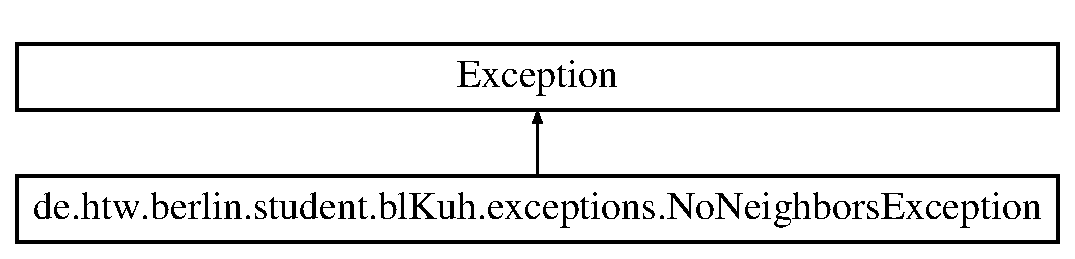
\includegraphics[height=2.000000cm]{classde_1_1htw_1_1berlin_1_1student_1_1bl_kuh_1_1exceptions_1_1_no_neighbors_exception}
\end{center}
\end{figure}
\subsection*{Public Member Functions}
\begin{DoxyCompactItemize}
\item 
\hyperlink{classde_1_1htw_1_1berlin_1_1student_1_1bl_kuh_1_1exceptions_1_1_no_neighbors_exception_ad6cd3043ac50230530d476426f8e462e}{No\-Neighbors\-Exception} (String message)
\end{DoxyCompactItemize}


\subsection{Detailed Description}
Exception to be thrown if the given tile has no neighbors.

\begin{DoxyAuthor}{Author}
Marcel Piater 
\end{DoxyAuthor}


\subsection{Constructor \& Destructor Documentation}
\hypertarget{classde_1_1htw_1_1berlin_1_1student_1_1bl_kuh_1_1exceptions_1_1_no_neighbors_exception_ad6cd3043ac50230530d476426f8e462e}{\index{de\-::htw\-::berlin\-::student\-::bl\-Kuh\-::exceptions\-::\-No\-Neighbors\-Exception@{de\-::htw\-::berlin\-::student\-::bl\-Kuh\-::exceptions\-::\-No\-Neighbors\-Exception}!No\-Neighbors\-Exception@{No\-Neighbors\-Exception}}
\index{No\-Neighbors\-Exception@{No\-Neighbors\-Exception}!de::htw::berlin::student::blKuh::exceptions::NoNeighborsException@{de\-::htw\-::berlin\-::student\-::bl\-Kuh\-::exceptions\-::\-No\-Neighbors\-Exception}}
\subsubsection[{No\-Neighbors\-Exception}]{\setlength{\rightskip}{0pt plus 5cm}de.\-htw.\-berlin.\-student.\-bl\-Kuh.\-exceptions.\-No\-Neighbors\-Exception.\-No\-Neighbors\-Exception (
\begin{DoxyParamCaption}
\item[{String}]{message}
\end{DoxyParamCaption}
)}}\label{classde_1_1htw_1_1berlin_1_1student_1_1bl_kuh_1_1exceptions_1_1_no_neighbors_exception_ad6cd3043ac50230530d476426f8e462e}
Constructor.


\begin{DoxyParams}{Parameters}
{\em message} & the message for the exception \\
\hline
\end{DoxyParams}


The documentation for this class was generated from the following file\-:\begin{DoxyCompactItemize}
\item 
D\-:/projects/bl\-Kuh/src/main/java/de/htw/berlin/student/bl\-Kuh/exceptions/\hyperlink{_no_neighbors_exception_8java}{No\-Neighbors\-Exception.\-java}\end{DoxyCompactItemize}

\hypertarget{classde_1_1htw_1_1berlin_1_1student_1_1bl_kuh_1_1view_1_1_options_view}{\section{de.\-htw.\-berlin.\-student.\-bl\-Kuh.\-view.\-Options\-View Class Reference}
\label{classde_1_1htw_1_1berlin_1_1student_1_1bl_kuh_1_1view_1_1_options_view}\index{de.\-htw.\-berlin.\-student.\-bl\-Kuh.\-view.\-Options\-View@{de.\-htw.\-berlin.\-student.\-bl\-Kuh.\-view.\-Options\-View}}
}
Inheritance diagram for de.\-htw.\-berlin.\-student.\-bl\-Kuh.\-view.\-Options\-View\-:\begin{figure}[H]
\begin{center}
\leavevmode
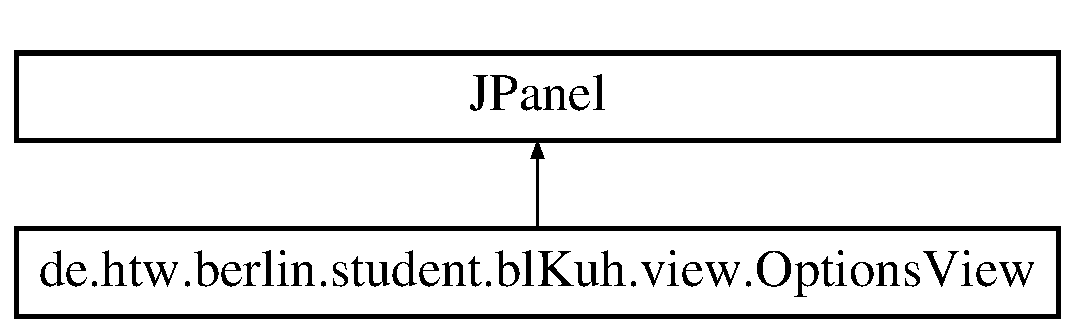
\includegraphics[height=2.000000cm]{classde_1_1htw_1_1berlin_1_1student_1_1bl_kuh_1_1view_1_1_options_view}
\end{center}
\end{figure}
\subsection*{Public Member Functions}
\begin{DoxyCompactItemize}
\item 
\hyperlink{classde_1_1htw_1_1berlin_1_1student_1_1bl_kuh_1_1view_1_1_options_view_af5ca1f039ea46744ee890c0bff34cf3b}{Options\-View} ()
\end{DoxyCompactItemize}


\subsection{Detailed Description}
A panel for the options view to adjust color and playground size.

\begin{DoxyAuthor}{Author}
Matthias Drummer $<$s0542834$>$ 

Marcel Piater 
\end{DoxyAuthor}


\subsection{Constructor \& Destructor Documentation}
\hypertarget{classde_1_1htw_1_1berlin_1_1student_1_1bl_kuh_1_1view_1_1_options_view_af5ca1f039ea46744ee890c0bff34cf3b}{\index{de\-::htw\-::berlin\-::student\-::bl\-Kuh\-::view\-::\-Options\-View@{de\-::htw\-::berlin\-::student\-::bl\-Kuh\-::view\-::\-Options\-View}!Options\-View@{Options\-View}}
\index{Options\-View@{Options\-View}!de::htw::berlin::student::blKuh::view::OptionsView@{de\-::htw\-::berlin\-::student\-::bl\-Kuh\-::view\-::\-Options\-View}}
\subsubsection[{Options\-View}]{\setlength{\rightskip}{0pt plus 5cm}de.\-htw.\-berlin.\-student.\-bl\-Kuh.\-view.\-Options\-View.\-Options\-View (
\begin{DoxyParamCaption}
{}
\end{DoxyParamCaption}
)}}\label{classde_1_1htw_1_1berlin_1_1student_1_1bl_kuh_1_1view_1_1_options_view_af5ca1f039ea46744ee890c0bff34cf3b}
Constructor. 

The documentation for this class was generated from the following file\-:\begin{DoxyCompactItemize}
\item 
D\-:/projects/bl\-Kuh/src/main/java/de/htw/berlin/student/bl\-Kuh/view/\hyperlink{_options_view_8java}{Options\-View.\-java}\end{DoxyCompactItemize}

\hypertarget{classbl_kuh_1_1_randomizer_test}{\section{bl\-Kuh.\-Randomizer\-Test Class Reference}
\label{classbl_kuh_1_1_randomizer_test}\index{bl\-Kuh.\-Randomizer\-Test@{bl\-Kuh.\-Randomizer\-Test}}
}
\subsection*{Public Member Functions}
\begin{DoxyCompactItemize}
\item 
void \hyperlink{classbl_kuh_1_1_randomizer_test_abef84bfd8761cdd7d3634eed149ec186}{test\-Randoms} ()
\end{DoxyCompactItemize}


\subsection{Member Function Documentation}
\hypertarget{classbl_kuh_1_1_randomizer_test_abef84bfd8761cdd7d3634eed149ec186}{\index{bl\-Kuh\-::\-Randomizer\-Test@{bl\-Kuh\-::\-Randomizer\-Test}!test\-Randoms@{test\-Randoms}}
\index{test\-Randoms@{test\-Randoms}!blKuh::RandomizerTest@{bl\-Kuh\-::\-Randomizer\-Test}}
\subsubsection[{test\-Randoms}]{\setlength{\rightskip}{0pt plus 5cm}void bl\-Kuh.\-Randomizer\-Test.\-test\-Randoms (
\begin{DoxyParamCaption}
{}
\end{DoxyParamCaption}
)}}\label{classbl_kuh_1_1_randomizer_test_abef84bfd8761cdd7d3634eed149ec186}


The documentation for this class was generated from the following file\-:\begin{DoxyCompactItemize}
\item 
D\-:/projects/bl\-Kuh/src/test/java/bl\-Kuh/\hyperlink{_randomizer_test_8java}{Randomizer\-Test.\-java}\end{DoxyCompactItemize}

\hypertarget{classde_1_1htw_1_1berlin_1_1student_1_1bl_kuh_1_1model_1_1_settings}{\section{de.\-htw.\-berlin.\-student.\-bl\-Kuh.\-model.\-Settings Class Reference}
\label{classde_1_1htw_1_1berlin_1_1student_1_1bl_kuh_1_1model_1_1_settings}\index{de.\-htw.\-berlin.\-student.\-bl\-Kuh.\-model.\-Settings@{de.\-htw.\-berlin.\-student.\-bl\-Kuh.\-model.\-Settings}}
}
\subsection*{Public Member Functions}
\begin{DoxyCompactItemize}
\item 
void \hyperlink{classde_1_1htw_1_1berlin_1_1student_1_1bl_kuh_1_1model_1_1_settings_a29999719759e8859463632d58d2051b0}{set\-Game\-Area\-Dimensions} (int dimension\-X, int dimension\-Y)
\item 
void \hyperlink{classde_1_1htw_1_1berlin_1_1student_1_1bl_kuh_1_1model_1_1_settings_a3728c011c35d4f6475d8b06eafb6d1c8}{set\-Colors\-To\-Use} (List$<$ Color $>$ colors\-To\-Use)
\item 
List$<$ Color $>$ \hyperlink{classde_1_1htw_1_1berlin_1_1student_1_1bl_kuh_1_1model_1_1_settings_ae73ab5e1b4bca3a5151d77f049ee5936}{get\-Colors\-To\-Use} ()
\item 
int \hyperlink{classde_1_1htw_1_1berlin_1_1student_1_1bl_kuh_1_1model_1_1_settings_afb5ad53400828d1c6b842c41a6a2f0b9}{get\-Dimension\-X} ()
\item 
int \hyperlink{classde_1_1htw_1_1berlin_1_1student_1_1bl_kuh_1_1model_1_1_settings_a913e9d831f39fed17d128657853e1e4d}{get\-Dimension\-Y} ()
\end{DoxyCompactItemize}
\subsection*{Static Public Member Functions}
\begin{DoxyCompactItemize}
\item 
static \hyperlink{classde_1_1htw_1_1berlin_1_1student_1_1bl_kuh_1_1model_1_1_settings}{Settings} \hyperlink{classde_1_1htw_1_1berlin_1_1student_1_1bl_kuh_1_1model_1_1_settings_a7e478e2ec72eba5a98a81e624c43cd8e}{get\-Instance} ()
\end{DoxyCompactItemize}


\subsection{Detailed Description}
A singleton object for settings.

\begin{DoxyAuthor}{Author}
Matthias Drummer $<$s0542834$>$ 
\end{DoxyAuthor}


\subsection{Member Function Documentation}
\hypertarget{classde_1_1htw_1_1berlin_1_1student_1_1bl_kuh_1_1model_1_1_settings_ae73ab5e1b4bca3a5151d77f049ee5936}{\index{de\-::htw\-::berlin\-::student\-::bl\-Kuh\-::model\-::\-Settings@{de\-::htw\-::berlin\-::student\-::bl\-Kuh\-::model\-::\-Settings}!get\-Colors\-To\-Use@{get\-Colors\-To\-Use}}
\index{get\-Colors\-To\-Use@{get\-Colors\-To\-Use}!de::htw::berlin::student::blKuh::model::Settings@{de\-::htw\-::berlin\-::student\-::bl\-Kuh\-::model\-::\-Settings}}
\subsubsection[{get\-Colors\-To\-Use}]{\setlength{\rightskip}{0pt plus 5cm}List$<$Color$>$ de.\-htw.\-berlin.\-student.\-bl\-Kuh.\-model.\-Settings.\-get\-Colors\-To\-Use (
\begin{DoxyParamCaption}
{}
\end{DoxyParamCaption}
)}}\label{classde_1_1htw_1_1berlin_1_1student_1_1bl_kuh_1_1model_1_1_settings_ae73ab5e1b4bca3a5151d77f049ee5936}
\hypertarget{classde_1_1htw_1_1berlin_1_1student_1_1bl_kuh_1_1model_1_1_settings_afb5ad53400828d1c6b842c41a6a2f0b9}{\index{de\-::htw\-::berlin\-::student\-::bl\-Kuh\-::model\-::\-Settings@{de\-::htw\-::berlin\-::student\-::bl\-Kuh\-::model\-::\-Settings}!get\-Dimension\-X@{get\-Dimension\-X}}
\index{get\-Dimension\-X@{get\-Dimension\-X}!de::htw::berlin::student::blKuh::model::Settings@{de\-::htw\-::berlin\-::student\-::bl\-Kuh\-::model\-::\-Settings}}
\subsubsection[{get\-Dimension\-X}]{\setlength{\rightskip}{0pt plus 5cm}int de.\-htw.\-berlin.\-student.\-bl\-Kuh.\-model.\-Settings.\-get\-Dimension\-X (
\begin{DoxyParamCaption}
{}
\end{DoxyParamCaption}
)}}\label{classde_1_1htw_1_1berlin_1_1student_1_1bl_kuh_1_1model_1_1_settings_afb5ad53400828d1c6b842c41a6a2f0b9}
\hypertarget{classde_1_1htw_1_1berlin_1_1student_1_1bl_kuh_1_1model_1_1_settings_a913e9d831f39fed17d128657853e1e4d}{\index{de\-::htw\-::berlin\-::student\-::bl\-Kuh\-::model\-::\-Settings@{de\-::htw\-::berlin\-::student\-::bl\-Kuh\-::model\-::\-Settings}!get\-Dimension\-Y@{get\-Dimension\-Y}}
\index{get\-Dimension\-Y@{get\-Dimension\-Y}!de::htw::berlin::student::blKuh::model::Settings@{de\-::htw\-::berlin\-::student\-::bl\-Kuh\-::model\-::\-Settings}}
\subsubsection[{get\-Dimension\-Y}]{\setlength{\rightskip}{0pt plus 5cm}int de.\-htw.\-berlin.\-student.\-bl\-Kuh.\-model.\-Settings.\-get\-Dimension\-Y (
\begin{DoxyParamCaption}
{}
\end{DoxyParamCaption}
)}}\label{classde_1_1htw_1_1berlin_1_1student_1_1bl_kuh_1_1model_1_1_settings_a913e9d831f39fed17d128657853e1e4d}
\hypertarget{classde_1_1htw_1_1berlin_1_1student_1_1bl_kuh_1_1model_1_1_settings_a7e478e2ec72eba5a98a81e624c43cd8e}{\index{de\-::htw\-::berlin\-::student\-::bl\-Kuh\-::model\-::\-Settings@{de\-::htw\-::berlin\-::student\-::bl\-Kuh\-::model\-::\-Settings}!get\-Instance@{get\-Instance}}
\index{get\-Instance@{get\-Instance}!de::htw::berlin::student::blKuh::model::Settings@{de\-::htw\-::berlin\-::student\-::bl\-Kuh\-::model\-::\-Settings}}
\subsubsection[{get\-Instance}]{\setlength{\rightskip}{0pt plus 5cm}static {\bf Settings} de.\-htw.\-berlin.\-student.\-bl\-Kuh.\-model.\-Settings.\-get\-Instance (
\begin{DoxyParamCaption}
{}
\end{DoxyParamCaption}
)\hspace{0.3cm}{\ttfamily [static]}}}\label{classde_1_1htw_1_1berlin_1_1student_1_1bl_kuh_1_1model_1_1_settings_a7e478e2ec72eba5a98a81e624c43cd8e}
Returns the settings instance.

\begin{DoxyReturn}{Returns}
the \hyperlink{classde_1_1htw_1_1berlin_1_1student_1_1bl_kuh_1_1model_1_1_settings}{Settings} instance. 
\end{DoxyReturn}
\hypertarget{classde_1_1htw_1_1berlin_1_1student_1_1bl_kuh_1_1model_1_1_settings_a3728c011c35d4f6475d8b06eafb6d1c8}{\index{de\-::htw\-::berlin\-::student\-::bl\-Kuh\-::model\-::\-Settings@{de\-::htw\-::berlin\-::student\-::bl\-Kuh\-::model\-::\-Settings}!set\-Colors\-To\-Use@{set\-Colors\-To\-Use}}
\index{set\-Colors\-To\-Use@{set\-Colors\-To\-Use}!de::htw::berlin::student::blKuh::model::Settings@{de\-::htw\-::berlin\-::student\-::bl\-Kuh\-::model\-::\-Settings}}
\subsubsection[{set\-Colors\-To\-Use}]{\setlength{\rightskip}{0pt plus 5cm}void de.\-htw.\-berlin.\-student.\-bl\-Kuh.\-model.\-Settings.\-set\-Colors\-To\-Use (
\begin{DoxyParamCaption}
\item[{List$<$ Color $>$}]{colors\-To\-Use}
\end{DoxyParamCaption}
)}}\label{classde_1_1htw_1_1berlin_1_1student_1_1bl_kuh_1_1model_1_1_settings_a3728c011c35d4f6475d8b06eafb6d1c8}
\hypertarget{classde_1_1htw_1_1berlin_1_1student_1_1bl_kuh_1_1model_1_1_settings_a29999719759e8859463632d58d2051b0}{\index{de\-::htw\-::berlin\-::student\-::bl\-Kuh\-::model\-::\-Settings@{de\-::htw\-::berlin\-::student\-::bl\-Kuh\-::model\-::\-Settings}!set\-Game\-Area\-Dimensions@{set\-Game\-Area\-Dimensions}}
\index{set\-Game\-Area\-Dimensions@{set\-Game\-Area\-Dimensions}!de::htw::berlin::student::blKuh::model::Settings@{de\-::htw\-::berlin\-::student\-::bl\-Kuh\-::model\-::\-Settings}}
\subsubsection[{set\-Game\-Area\-Dimensions}]{\setlength{\rightskip}{0pt plus 5cm}void de.\-htw.\-berlin.\-student.\-bl\-Kuh.\-model.\-Settings.\-set\-Game\-Area\-Dimensions (
\begin{DoxyParamCaption}
\item[{int}]{dimension\-X, }
\item[{int}]{dimension\-Y}
\end{DoxyParamCaption}
)}}\label{classde_1_1htw_1_1berlin_1_1student_1_1bl_kuh_1_1model_1_1_settings_a29999719759e8859463632d58d2051b0}


The documentation for this class was generated from the following file\-:\begin{DoxyCompactItemize}
\item 
D\-:/projects/bl\-Kuh/src/main/java/de/htw/berlin/student/bl\-Kuh/model/\hyperlink{_settings_8java}{Settings.\-java}\end{DoxyCompactItemize}

\hypertarget{classde_1_1htw_1_1berlin_1_1student_1_1bl_kuh_1_1_spielfeld}{\section{de.\-htw.\-berlin.\-student.\-bl\-Kuh.\-Spielfeld Class Reference}
\label{classde_1_1htw_1_1berlin_1_1student_1_1bl_kuh_1_1_spielfeld}\index{de.\-htw.\-berlin.\-student.\-bl\-Kuh.\-Spielfeld@{de.\-htw.\-berlin.\-student.\-bl\-Kuh.\-Spielfeld}}
}
\subsection*{Public Member Functions}
\begin{DoxyCompactItemize}
\item 
\hyperlink{classde_1_1htw_1_1berlin_1_1student_1_1bl_kuh_1_1_spielfeld_ae2a4fe2c5a8ba37144ee6e48ac3242c0}{Spielfeld} ()
\item 
void \hyperlink{classde_1_1htw_1_1berlin_1_1student_1_1bl_kuh_1_1_spielfeld_a940bddf1c60f46be6fe3852310b5706a}{generate} ()
\item 
void \hyperlink{classde_1_1htw_1_1berlin_1_1student_1_1bl_kuh_1_1_spielfeld_af35fcbf80ea3473ccf5316e55a1c33cf}{undo} ()
\item 
void \hyperlink{classde_1_1htw_1_1berlin_1_1student_1_1bl_kuh_1_1_spielfeld_a6492de4780cd44b168c89149172cd128}{perform\-Button\-Click} (int choord\-X, int choord\-Y)  throws No\-Neighbors\-Exception 
\item 
Color\mbox{[}$\,$\mbox{]}\mbox{[}$\,$\mbox{]} \hyperlink{classde_1_1htw_1_1berlin_1_1student_1_1bl_kuh_1_1_spielfeld_ad0318e304b73c0cad0476f1876a237d0}{get\-Matrix} ()
\item 
int \hyperlink{classde_1_1htw_1_1berlin_1_1student_1_1bl_kuh_1_1_spielfeld_a1961def0836db962975d8c367744def1}{get\-Points} ()
\item 
Boolean \hyperlink{classde_1_1htw_1_1berlin_1_1student_1_1bl_kuh_1_1_spielfeld_a02eba651e3ffcec3f707a57520da4c97}{has\-Moves\-Left} ()
\end{DoxyCompactItemize}


\subsection{Detailed Description}
Class that holds the playground data and calculate its state when events happen.

\begin{DoxyAuthor}{Author}
Matthias Drummer 

Marcel Piater 
\end{DoxyAuthor}


\subsection{Constructor \& Destructor Documentation}
\hypertarget{classde_1_1htw_1_1berlin_1_1student_1_1bl_kuh_1_1_spielfeld_ae2a4fe2c5a8ba37144ee6e48ac3242c0}{\index{de\-::htw\-::berlin\-::student\-::bl\-Kuh\-::\-Spielfeld@{de\-::htw\-::berlin\-::student\-::bl\-Kuh\-::\-Spielfeld}!Spielfeld@{Spielfeld}}
\index{Spielfeld@{Spielfeld}!de::htw::berlin::student::blKuh::Spielfeld@{de\-::htw\-::berlin\-::student\-::bl\-Kuh\-::\-Spielfeld}}
\subsubsection[{Spielfeld}]{\setlength{\rightskip}{0pt plus 5cm}de.\-htw.\-berlin.\-student.\-bl\-Kuh.\-Spielfeld.\-Spielfeld (
\begin{DoxyParamCaption}
{}
\end{DoxyParamCaption}
)}}\label{classde_1_1htw_1_1berlin_1_1student_1_1bl_kuh_1_1_spielfeld_ae2a4fe2c5a8ba37144ee6e48ac3242c0}
Default constructor. 

\subsection{Member Function Documentation}
\hypertarget{classde_1_1htw_1_1berlin_1_1student_1_1bl_kuh_1_1_spielfeld_a940bddf1c60f46be6fe3852310b5706a}{\index{de\-::htw\-::berlin\-::student\-::bl\-Kuh\-::\-Spielfeld@{de\-::htw\-::berlin\-::student\-::bl\-Kuh\-::\-Spielfeld}!generate@{generate}}
\index{generate@{generate}!de::htw::berlin::student::blKuh::Spielfeld@{de\-::htw\-::berlin\-::student\-::bl\-Kuh\-::\-Spielfeld}}
\subsubsection[{generate}]{\setlength{\rightskip}{0pt plus 5cm}void de.\-htw.\-berlin.\-student.\-bl\-Kuh.\-Spielfeld.\-generate (
\begin{DoxyParamCaption}
{}
\end{DoxyParamCaption}
)}}\label{classde_1_1htw_1_1berlin_1_1student_1_1bl_kuh_1_1_spielfeld_a940bddf1c60f46be6fe3852310b5706a}
\hypertarget{classde_1_1htw_1_1berlin_1_1student_1_1bl_kuh_1_1_spielfeld_ad0318e304b73c0cad0476f1876a237d0}{\index{de\-::htw\-::berlin\-::student\-::bl\-Kuh\-::\-Spielfeld@{de\-::htw\-::berlin\-::student\-::bl\-Kuh\-::\-Spielfeld}!get\-Matrix@{get\-Matrix}}
\index{get\-Matrix@{get\-Matrix}!de::htw::berlin::student::blKuh::Spielfeld@{de\-::htw\-::berlin\-::student\-::bl\-Kuh\-::\-Spielfeld}}
\subsubsection[{get\-Matrix}]{\setlength{\rightskip}{0pt plus 5cm}Color \mbox{[}$\,$\mbox{]}\mbox{[}$\,$\mbox{]} de.\-htw.\-berlin.\-student.\-bl\-Kuh.\-Spielfeld.\-get\-Matrix (
\begin{DoxyParamCaption}
{}
\end{DoxyParamCaption}
)}}\label{classde_1_1htw_1_1berlin_1_1student_1_1bl_kuh_1_1_spielfeld_ad0318e304b73c0cad0476f1876a237d0}
\hypertarget{classde_1_1htw_1_1berlin_1_1student_1_1bl_kuh_1_1_spielfeld_a1961def0836db962975d8c367744def1}{\index{de\-::htw\-::berlin\-::student\-::bl\-Kuh\-::\-Spielfeld@{de\-::htw\-::berlin\-::student\-::bl\-Kuh\-::\-Spielfeld}!get\-Points@{get\-Points}}
\index{get\-Points@{get\-Points}!de::htw::berlin::student::blKuh::Spielfeld@{de\-::htw\-::berlin\-::student\-::bl\-Kuh\-::\-Spielfeld}}
\subsubsection[{get\-Points}]{\setlength{\rightskip}{0pt plus 5cm}int de.\-htw.\-berlin.\-student.\-bl\-Kuh.\-Spielfeld.\-get\-Points (
\begin{DoxyParamCaption}
{}
\end{DoxyParamCaption}
)}}\label{classde_1_1htw_1_1berlin_1_1student_1_1bl_kuh_1_1_spielfeld_a1961def0836db962975d8c367744def1}
Returns the current points.

\begin{DoxyReturn}{Returns}
the points 
\end{DoxyReturn}
\hypertarget{classde_1_1htw_1_1berlin_1_1student_1_1bl_kuh_1_1_spielfeld_a02eba651e3ffcec3f707a57520da4c97}{\index{de\-::htw\-::berlin\-::student\-::bl\-Kuh\-::\-Spielfeld@{de\-::htw\-::berlin\-::student\-::bl\-Kuh\-::\-Spielfeld}!has\-Moves\-Left@{has\-Moves\-Left}}
\index{has\-Moves\-Left@{has\-Moves\-Left}!de::htw::berlin::student::blKuh::Spielfeld@{de\-::htw\-::berlin\-::student\-::bl\-Kuh\-::\-Spielfeld}}
\subsubsection[{has\-Moves\-Left}]{\setlength{\rightskip}{0pt plus 5cm}Boolean de.\-htw.\-berlin.\-student.\-bl\-Kuh.\-Spielfeld.\-has\-Moves\-Left (
\begin{DoxyParamCaption}
{}
\end{DoxyParamCaption}
)}}\label{classde_1_1htw_1_1berlin_1_1student_1_1bl_kuh_1_1_spielfeld_a02eba651e3ffcec3f707a57520da4c97}
Checks if there are any moves left to be performed.

\begin{DoxyReturn}{Returns}
true if there are moves left, false if there are no more moves and null if the game is won. 
\end{DoxyReturn}
\hypertarget{classde_1_1htw_1_1berlin_1_1student_1_1bl_kuh_1_1_spielfeld_a6492de4780cd44b168c89149172cd128}{\index{de\-::htw\-::berlin\-::student\-::bl\-Kuh\-::\-Spielfeld@{de\-::htw\-::berlin\-::student\-::bl\-Kuh\-::\-Spielfeld}!perform\-Button\-Click@{perform\-Button\-Click}}
\index{perform\-Button\-Click@{perform\-Button\-Click}!de::htw::berlin::student::blKuh::Spielfeld@{de\-::htw\-::berlin\-::student\-::bl\-Kuh\-::\-Spielfeld}}
\subsubsection[{perform\-Button\-Click}]{\setlength{\rightskip}{0pt plus 5cm}void de.\-htw.\-berlin.\-student.\-bl\-Kuh.\-Spielfeld.\-perform\-Button\-Click (
\begin{DoxyParamCaption}
\item[{int}]{choord\-X, }
\item[{int}]{choord\-Y}
\end{DoxyParamCaption}
) throws {\bf No\-Neighbors\-Exception}}}\label{classde_1_1htw_1_1berlin_1_1student_1_1bl_kuh_1_1_spielfeld_a6492de4780cd44b168c89149172cd128}
Method called when one tile has been clicked. The points are counted and an undo matrix is created.


\begin{DoxyParams}{Parameters}
{\em choord\-X} & the x coordinate of the tile which has been clicked \\
\hline
{\em choord\-Y} & the y coordinate of the tile which has been clicked \\
\hline
\end{DoxyParams}

\begin{DoxyExceptions}{Exceptions}
{\em No\-Neighbors\-Exception} & thrown if there are no neighbors nearby the clicked tile. \\
\hline
\end{DoxyExceptions}
\hypertarget{classde_1_1htw_1_1berlin_1_1student_1_1bl_kuh_1_1_spielfeld_af35fcbf80ea3473ccf5316e55a1c33cf}{\index{de\-::htw\-::berlin\-::student\-::bl\-Kuh\-::\-Spielfeld@{de\-::htw\-::berlin\-::student\-::bl\-Kuh\-::\-Spielfeld}!undo@{undo}}
\index{undo@{undo}!de::htw::berlin::student::blKuh::Spielfeld@{de\-::htw\-::berlin\-::student\-::bl\-Kuh\-::\-Spielfeld}}
\subsubsection[{undo}]{\setlength{\rightskip}{0pt plus 5cm}void de.\-htw.\-berlin.\-student.\-bl\-Kuh.\-Spielfeld.\-undo (
\begin{DoxyParamCaption}
{}
\end{DoxyParamCaption}
)}}\label{classde_1_1htw_1_1berlin_1_1student_1_1bl_kuh_1_1_spielfeld_af35fcbf80ea3473ccf5316e55a1c33cf}
Undoes one step if possible. 

The documentation for this class was generated from the following file\-:\begin{DoxyCompactItemize}
\item 
D\-:/projects/bl\-Kuh/src/main/java/de/htw/berlin/student/bl\-Kuh/\hyperlink{_spielfeld_8java}{Spielfeld.\-java}\end{DoxyCompactItemize}

\hypertarget{classde_1_1htw_1_1berlin_1_1student_1_1bl_kuh_1_1view_1_1_spielfeld_view}{\section{de.\-htw.\-berlin.\-student.\-bl\-Kuh.\-view.\-Spielfeld\-View Class Reference}
\label{classde_1_1htw_1_1berlin_1_1student_1_1bl_kuh_1_1view_1_1_spielfeld_view}\index{de.\-htw.\-berlin.\-student.\-bl\-Kuh.\-view.\-Spielfeld\-View@{de.\-htw.\-berlin.\-student.\-bl\-Kuh.\-view.\-Spielfeld\-View}}
}
Inheritance diagram for de.\-htw.\-berlin.\-student.\-bl\-Kuh.\-view.\-Spielfeld\-View\-:\begin{figure}[H]
\begin{center}
\leavevmode
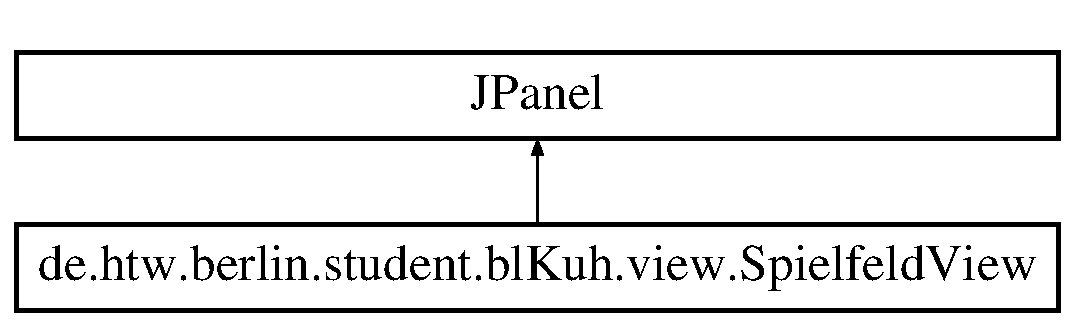
\includegraphics[height=2.000000cm]{classde_1_1htw_1_1berlin_1_1student_1_1bl_kuh_1_1view_1_1_spielfeld_view}
\end{center}
\end{figure}
\subsection*{Public Member Functions}
\begin{DoxyCompactItemize}
\item 
\hyperlink{classde_1_1htw_1_1berlin_1_1student_1_1bl_kuh_1_1view_1_1_spielfeld_view_aae3ce674647d9ab92b66316a0a82bbdd}{Spielfeld\-View} (Color\mbox{[}$\,$\mbox{]}\mbox{[}$\,$\mbox{]} matrix)
\item 
void \hyperlink{classde_1_1htw_1_1berlin_1_1student_1_1bl_kuh_1_1view_1_1_spielfeld_view_aed88286402a54ce980ddd84bf7ae98f1}{set\-Points} (int points)
\item 
void \hyperlink{classde_1_1htw_1_1berlin_1_1student_1_1bl_kuh_1_1view_1_1_spielfeld_view_ac129b0ada7f675559817c204ff7dec8d}{rebuild} (Color\mbox{[}$\,$\mbox{]}\mbox{[}$\,$\mbox{]} matrix)
\item 
void \hyperlink{classde_1_1htw_1_1berlin_1_1student_1_1bl_kuh_1_1view_1_1_spielfeld_view_a9ba63fc014f1a849064738d43d718a74}{set\-Tile\-Clicked\-Action\-Listener} (Action\-Listener tile\-Clicked\-Action\-Listener)
\end{DoxyCompactItemize}


\subsection{Detailed Description}
A view panel that displays the playground that consists of clickable buttons and displays the gained points.

\begin{DoxyAuthor}{Author}
Matthias Drummer 

Marcel Piater 
\end{DoxyAuthor}


\subsection{Constructor \& Destructor Documentation}
\hypertarget{classde_1_1htw_1_1berlin_1_1student_1_1bl_kuh_1_1view_1_1_spielfeld_view_aae3ce674647d9ab92b66316a0a82bbdd}{\index{de\-::htw\-::berlin\-::student\-::bl\-Kuh\-::view\-::\-Spielfeld\-View@{de\-::htw\-::berlin\-::student\-::bl\-Kuh\-::view\-::\-Spielfeld\-View}!Spielfeld\-View@{Spielfeld\-View}}
\index{Spielfeld\-View@{Spielfeld\-View}!de::htw::berlin::student::blKuh::view::SpielfeldView@{de\-::htw\-::berlin\-::student\-::bl\-Kuh\-::view\-::\-Spielfeld\-View}}
\subsubsection[{Spielfeld\-View}]{\setlength{\rightskip}{0pt plus 5cm}de.\-htw.\-berlin.\-student.\-bl\-Kuh.\-view.\-Spielfeld\-View.\-Spielfeld\-View (
\begin{DoxyParamCaption}
\item[{Color}]{matrix\mbox{[}$\,$\mbox{]}\mbox{[}$\,$\mbox{]}}
\end{DoxyParamCaption}
)}}\label{classde_1_1htw_1_1berlin_1_1student_1_1bl_kuh_1_1view_1_1_spielfeld_view_aae3ce674647d9ab92b66316a0a82bbdd}
Constructor.


\begin{DoxyParams}{Parameters}
{\em matrix} & a two dimensional array of type color which represents our playground. \\
\hline
\end{DoxyParams}


\subsection{Member Function Documentation}
\hypertarget{classde_1_1htw_1_1berlin_1_1student_1_1bl_kuh_1_1view_1_1_spielfeld_view_ac129b0ada7f675559817c204ff7dec8d}{\index{de\-::htw\-::berlin\-::student\-::bl\-Kuh\-::view\-::\-Spielfeld\-View@{de\-::htw\-::berlin\-::student\-::bl\-Kuh\-::view\-::\-Spielfeld\-View}!rebuild@{rebuild}}
\index{rebuild@{rebuild}!de::htw::berlin::student::blKuh::view::SpielfeldView@{de\-::htw\-::berlin\-::student\-::bl\-Kuh\-::view\-::\-Spielfeld\-View}}
\subsubsection[{rebuild}]{\setlength{\rightskip}{0pt plus 5cm}void de.\-htw.\-berlin.\-student.\-bl\-Kuh.\-view.\-Spielfeld\-View.\-rebuild (
\begin{DoxyParamCaption}
\item[{Color}]{matrix\mbox{[}$\,$\mbox{]}\mbox{[}$\,$\mbox{]}}
\end{DoxyParamCaption}
)}}\label{classde_1_1htw_1_1berlin_1_1student_1_1bl_kuh_1_1view_1_1_spielfeld_view_ac129b0ada7f675559817c204ff7dec8d}
Rebuilds the visible playground with the values given by the color matrix.


\begin{DoxyParams}{Parameters}
{\em matrix} & the playground area as two dimensional color array \\
\hline
\end{DoxyParams}
\hypertarget{classde_1_1htw_1_1berlin_1_1student_1_1bl_kuh_1_1view_1_1_spielfeld_view_aed88286402a54ce980ddd84bf7ae98f1}{\index{de\-::htw\-::berlin\-::student\-::bl\-Kuh\-::view\-::\-Spielfeld\-View@{de\-::htw\-::berlin\-::student\-::bl\-Kuh\-::view\-::\-Spielfeld\-View}!set\-Points@{set\-Points}}
\index{set\-Points@{set\-Points}!de::htw::berlin::student::blKuh::view::SpielfeldView@{de\-::htw\-::berlin\-::student\-::bl\-Kuh\-::view\-::\-Spielfeld\-View}}
\subsubsection[{set\-Points}]{\setlength{\rightskip}{0pt plus 5cm}void de.\-htw.\-berlin.\-student.\-bl\-Kuh.\-view.\-Spielfeld\-View.\-set\-Points (
\begin{DoxyParamCaption}
\item[{int}]{points}
\end{DoxyParamCaption}
)}}\label{classde_1_1htw_1_1berlin_1_1student_1_1bl_kuh_1_1view_1_1_spielfeld_view_aed88286402a54ce980ddd84bf7ae98f1}
Sets the points to the label.


\begin{DoxyParams}{Parameters}
{\em points} & \\
\hline
\end{DoxyParams}
\hypertarget{classde_1_1htw_1_1berlin_1_1student_1_1bl_kuh_1_1view_1_1_spielfeld_view_a9ba63fc014f1a849064738d43d718a74}{\index{de\-::htw\-::berlin\-::student\-::bl\-Kuh\-::view\-::\-Spielfeld\-View@{de\-::htw\-::berlin\-::student\-::bl\-Kuh\-::view\-::\-Spielfeld\-View}!set\-Tile\-Clicked\-Action\-Listener@{set\-Tile\-Clicked\-Action\-Listener}}
\index{set\-Tile\-Clicked\-Action\-Listener@{set\-Tile\-Clicked\-Action\-Listener}!de::htw::berlin::student::blKuh::view::SpielfeldView@{de\-::htw\-::berlin\-::student\-::bl\-Kuh\-::view\-::\-Spielfeld\-View}}
\subsubsection[{set\-Tile\-Clicked\-Action\-Listener}]{\setlength{\rightskip}{0pt plus 5cm}void de.\-htw.\-berlin.\-student.\-bl\-Kuh.\-view.\-Spielfeld\-View.\-set\-Tile\-Clicked\-Action\-Listener (
\begin{DoxyParamCaption}
\item[{Action\-Listener}]{tile\-Clicked\-Action\-Listener}
\end{DoxyParamCaption}
)}}\label{classde_1_1htw_1_1berlin_1_1student_1_1bl_kuh_1_1view_1_1_spielfeld_view_a9ba63fc014f1a849064738d43d718a74}
Sets the tile clicked action listener. It will fire an event when a button has been clicked.


\begin{DoxyParams}{Parameters}
{\em tile\-Clicked\-Action\-Listener} & the tile\-Clicked\-Action\-Listener \\
\hline
\end{DoxyParams}


The documentation for this class was generated from the following file\-:\begin{DoxyCompactItemize}
\item 
D\-:/projects/bl\-Kuh/src/main/java/de/htw/berlin/student/bl\-Kuh/view/\hyperlink{_spielfeld_view_8java}{Spielfeld\-View.\-java}\end{DoxyCompactItemize}

\hypertarget{classde_1_1htw_1_1berlin_1_1student_1_1bl_kuh_1_1component_1_1_tile_button}{\section{de.\-htw.\-berlin.\-student.\-bl\-Kuh.\-component.\-Tile\-Button Class Reference}
\label{classde_1_1htw_1_1berlin_1_1student_1_1bl_kuh_1_1component_1_1_tile_button}\index{de.\-htw.\-berlin.\-student.\-bl\-Kuh.\-component.\-Tile\-Button@{de.\-htw.\-berlin.\-student.\-bl\-Kuh.\-component.\-Tile\-Button}}
}
Inheritance diagram for de.\-htw.\-berlin.\-student.\-bl\-Kuh.\-component.\-Tile\-Button\-:\begin{figure}[H]
\begin{center}
\leavevmode
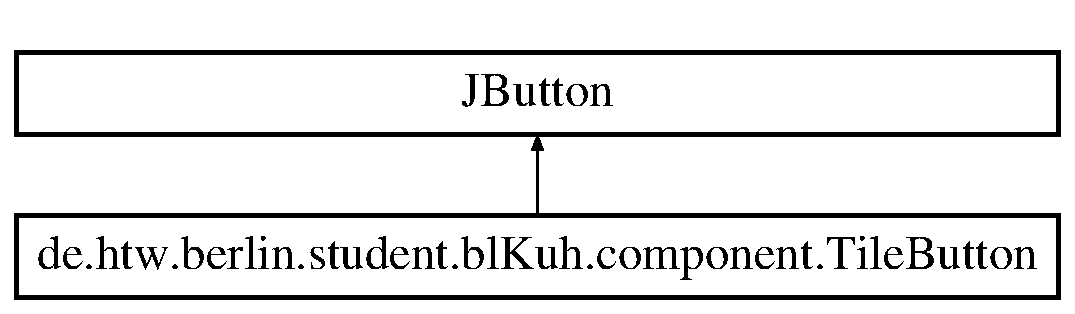
\includegraphics[height=2.000000cm]{classde_1_1htw_1_1berlin_1_1student_1_1bl_kuh_1_1component_1_1_tile_button}
\end{center}
\end{figure}
\subsection*{Public Member Functions}
\begin{DoxyCompactItemize}
\item 
\hyperlink{classde_1_1htw_1_1berlin_1_1student_1_1bl_kuh_1_1component_1_1_tile_button_ab02c4c2ca599f6f4d08aa8a57c351a71}{Tile\-Button} (int choordinate\-X, int choordinate\-Y, Color color)
\item 
int \hyperlink{classde_1_1htw_1_1berlin_1_1student_1_1bl_kuh_1_1component_1_1_tile_button_a32580865b121cbc59472ae5e2b0348a6}{get\-Choordinate\-X} ()
\item 
int \hyperlink{classde_1_1htw_1_1berlin_1_1student_1_1bl_kuh_1_1component_1_1_tile_button_a287a0da19012b7900abee3b6ade5333d}{get\-Choordinate\-Y} ()
\item 
String \hyperlink{classde_1_1htw_1_1berlin_1_1student_1_1bl_kuh_1_1component_1_1_tile_button_aa10ff18fab436932ecca9aa42c141776}{to\-String} ()
\end{DoxyCompactItemize}


\subsection{Detailed Description}
A class for the tile.

\begin{DoxyAuthor}{Author}
Matthias Drummer 
\end{DoxyAuthor}


\subsection{Constructor \& Destructor Documentation}
\hypertarget{classde_1_1htw_1_1berlin_1_1student_1_1bl_kuh_1_1component_1_1_tile_button_ab02c4c2ca599f6f4d08aa8a57c351a71}{\index{de\-::htw\-::berlin\-::student\-::bl\-Kuh\-::component\-::\-Tile\-Button@{de\-::htw\-::berlin\-::student\-::bl\-Kuh\-::component\-::\-Tile\-Button}!Tile\-Button@{Tile\-Button}}
\index{Tile\-Button@{Tile\-Button}!de::htw::berlin::student::blKuh::component::TileButton@{de\-::htw\-::berlin\-::student\-::bl\-Kuh\-::component\-::\-Tile\-Button}}
\subsubsection[{Tile\-Button}]{\setlength{\rightskip}{0pt plus 5cm}de.\-htw.\-berlin.\-student.\-bl\-Kuh.\-component.\-Tile\-Button.\-Tile\-Button (
\begin{DoxyParamCaption}
\item[{int}]{choordinate\-X, }
\item[{int}]{choordinate\-Y, }
\item[{Color}]{color}
\end{DoxyParamCaption}
)}}\label{classde_1_1htw_1_1berlin_1_1student_1_1bl_kuh_1_1component_1_1_tile_button_ab02c4c2ca599f6f4d08aa8a57c351a71}
Constructor


\begin{DoxyParams}{Parameters}
{\em choordinate\-X} & the index for the x value \\
\hline
{\em choordinate\-Y} & the index for the y value \\
\hline
{\em color} & the color of the tile \\
\hline
\end{DoxyParams}


\subsection{Member Function Documentation}
\hypertarget{classde_1_1htw_1_1berlin_1_1student_1_1bl_kuh_1_1component_1_1_tile_button_a32580865b121cbc59472ae5e2b0348a6}{\index{de\-::htw\-::berlin\-::student\-::bl\-Kuh\-::component\-::\-Tile\-Button@{de\-::htw\-::berlin\-::student\-::bl\-Kuh\-::component\-::\-Tile\-Button}!get\-Choordinate\-X@{get\-Choordinate\-X}}
\index{get\-Choordinate\-X@{get\-Choordinate\-X}!de::htw::berlin::student::blKuh::component::TileButton@{de\-::htw\-::berlin\-::student\-::bl\-Kuh\-::component\-::\-Tile\-Button}}
\subsubsection[{get\-Choordinate\-X}]{\setlength{\rightskip}{0pt plus 5cm}int de.\-htw.\-berlin.\-student.\-bl\-Kuh.\-component.\-Tile\-Button.\-get\-Choordinate\-X (
\begin{DoxyParamCaption}
{}
\end{DoxyParamCaption}
)}}\label{classde_1_1htw_1_1berlin_1_1student_1_1bl_kuh_1_1component_1_1_tile_button_a32580865b121cbc59472ae5e2b0348a6}
\hypertarget{classde_1_1htw_1_1berlin_1_1student_1_1bl_kuh_1_1component_1_1_tile_button_a287a0da19012b7900abee3b6ade5333d}{\index{de\-::htw\-::berlin\-::student\-::bl\-Kuh\-::component\-::\-Tile\-Button@{de\-::htw\-::berlin\-::student\-::bl\-Kuh\-::component\-::\-Tile\-Button}!get\-Choordinate\-Y@{get\-Choordinate\-Y}}
\index{get\-Choordinate\-Y@{get\-Choordinate\-Y}!de::htw::berlin::student::blKuh::component::TileButton@{de\-::htw\-::berlin\-::student\-::bl\-Kuh\-::component\-::\-Tile\-Button}}
\subsubsection[{get\-Choordinate\-Y}]{\setlength{\rightskip}{0pt plus 5cm}int de.\-htw.\-berlin.\-student.\-bl\-Kuh.\-component.\-Tile\-Button.\-get\-Choordinate\-Y (
\begin{DoxyParamCaption}
{}
\end{DoxyParamCaption}
)}}\label{classde_1_1htw_1_1berlin_1_1student_1_1bl_kuh_1_1component_1_1_tile_button_a287a0da19012b7900abee3b6ade5333d}
\hypertarget{classde_1_1htw_1_1berlin_1_1student_1_1bl_kuh_1_1component_1_1_tile_button_aa10ff18fab436932ecca9aa42c141776}{\index{de\-::htw\-::berlin\-::student\-::bl\-Kuh\-::component\-::\-Tile\-Button@{de\-::htw\-::berlin\-::student\-::bl\-Kuh\-::component\-::\-Tile\-Button}!to\-String@{to\-String}}
\index{to\-String@{to\-String}!de::htw::berlin::student::blKuh::component::TileButton@{de\-::htw\-::berlin\-::student\-::bl\-Kuh\-::component\-::\-Tile\-Button}}
\subsubsection[{to\-String}]{\setlength{\rightskip}{0pt plus 5cm}String de.\-htw.\-berlin.\-student.\-bl\-Kuh.\-component.\-Tile\-Button.\-to\-String (
\begin{DoxyParamCaption}
{}
\end{DoxyParamCaption}
)}}\label{classde_1_1htw_1_1berlin_1_1student_1_1bl_kuh_1_1component_1_1_tile_button_aa10ff18fab436932ecca9aa42c141776}


The documentation for this class was generated from the following file\-:\begin{DoxyCompactItemize}
\item 
D\-:/projects/bl\-Kuh/src/main/java/de/htw/berlin/student/bl\-Kuh/component/\hyperlink{_tile_button_8java}{Tile\-Button.\-java}\end{DoxyCompactItemize}

\chapter{File Documentation}
\hypertarget{_r_e_a_d_m_e_8md}{\section{D\-:/projects/bl\-Kuh/\-R\-E\-A\-D\-M\-E.md File Reference}
\label{_r_e_a_d_m_e_8md}\index{D\-:/projects/bl\-Kuh/\-R\-E\-A\-D\-M\-E.\-md@{D\-:/projects/bl\-Kuh/\-R\-E\-A\-D\-M\-E.\-md}}
}

\hypertarget{_tile_button_8java}{\section{D\-:/projects/bl\-Kuh/src/main/java/de/htw/berlin/student/bl\-Kuh/component/\-Tile\-Button.java File Reference}
\label{_tile_button_8java}\index{D\-:/projects/bl\-Kuh/src/main/java/de/htw/berlin/student/bl\-Kuh/component/\-Tile\-Button.\-java@{D\-:/projects/bl\-Kuh/src/main/java/de/htw/berlin/student/bl\-Kuh/component/\-Tile\-Button.\-java}}
}
\subsection*{Classes}
\begin{DoxyCompactItemize}
\item 
class \hyperlink{classde_1_1htw_1_1berlin_1_1student_1_1bl_kuh_1_1component_1_1_tile_button}{de.\-htw.\-berlin.\-student.\-bl\-Kuh.\-component.\-Tile\-Button}
\end{DoxyCompactItemize}
\subsection*{Packages}
\begin{DoxyCompactItemize}
\item 
package \hyperlink{namespacede_1_1htw_1_1berlin_1_1student_1_1bl_kuh_1_1component}{de.\-htw.\-berlin.\-student.\-bl\-Kuh.\-component}
\end{DoxyCompactItemize}

\hypertarget{_no_neighbors_exception_8java}{\section{D\-:/projects/bl\-Kuh/src/main/java/de/htw/berlin/student/bl\-Kuh/exceptions/\-No\-Neighbors\-Exception.java File Reference}
\label{_no_neighbors_exception_8java}\index{D\-:/projects/bl\-Kuh/src/main/java/de/htw/berlin/student/bl\-Kuh/exceptions/\-No\-Neighbors\-Exception.\-java@{D\-:/projects/bl\-Kuh/src/main/java/de/htw/berlin/student/bl\-Kuh/exceptions/\-No\-Neighbors\-Exception.\-java}}
}
\subsection*{Classes}
\begin{DoxyCompactItemize}
\item 
class \hyperlink{classde_1_1htw_1_1berlin_1_1student_1_1bl_kuh_1_1exceptions_1_1_no_neighbors_exception}{de.\-htw.\-berlin.\-student.\-bl\-Kuh.\-exceptions.\-No\-Neighbors\-Exception}
\end{DoxyCompactItemize}
\subsection*{Packages}
\begin{DoxyCompactItemize}
\item 
package \hyperlink{namespacede_1_1htw_1_1berlin_1_1student_1_1bl_kuh_1_1exceptions}{de.\-htw.\-berlin.\-student.\-bl\-Kuh.\-exceptions}
\end{DoxyCompactItemize}

\hypertarget{_main_8java}{\section{D\-:/projects/bl\-Kuh/src/main/java/de/htw/berlin/student/bl\-Kuh/\-Main.java File Reference}
\label{_main_8java}\index{D\-:/projects/bl\-Kuh/src/main/java/de/htw/berlin/student/bl\-Kuh/\-Main.\-java@{D\-:/projects/bl\-Kuh/src/main/java/de/htw/berlin/student/bl\-Kuh/\-Main.\-java}}
}
\subsection*{Classes}
\begin{DoxyCompactItemize}
\item 
class \hyperlink{classde_1_1htw_1_1berlin_1_1student_1_1bl_kuh_1_1_main}{de.\-htw.\-berlin.\-student.\-bl\-Kuh.\-Main}
\end{DoxyCompactItemize}
\subsection*{Packages}
\begin{DoxyCompactItemize}
\item 
package \hyperlink{namespacede_1_1htw_1_1berlin_1_1student_1_1bl_kuh}{de.\-htw.\-berlin.\-student.\-bl\-Kuh}
\end{DoxyCompactItemize}

\hypertarget{_main_window_8java}{\section{D\-:/projects/bl\-Kuh/src/main/java/de/htw/berlin/student/bl\-Kuh/\-Main\-Window.java File Reference}
\label{_main_window_8java}\index{D\-:/projects/bl\-Kuh/src/main/java/de/htw/berlin/student/bl\-Kuh/\-Main\-Window.\-java@{D\-:/projects/bl\-Kuh/src/main/java/de/htw/berlin/student/bl\-Kuh/\-Main\-Window.\-java}}
}
\subsection*{Classes}
\begin{DoxyCompactItemize}
\item 
class \hyperlink{classde_1_1htw_1_1berlin_1_1student_1_1bl_kuh_1_1_main_window}{de.\-htw.\-berlin.\-student.\-bl\-Kuh.\-Main\-Window}
\end{DoxyCompactItemize}
\subsection*{Packages}
\begin{DoxyCompactItemize}
\item 
package \hyperlink{namespacede_1_1htw_1_1berlin_1_1student_1_1bl_kuh}{de.\-htw.\-berlin.\-student.\-bl\-Kuh}
\end{DoxyCompactItemize}

\hypertarget{_menu_items_8java}{\section{D\-:/projects/bl\-Kuh/src/main/java/de/htw/berlin/student/bl\-Kuh/menu/\-Menu\-Items.java File Reference}
\label{_menu_items_8java}\index{D\-:/projects/bl\-Kuh/src/main/java/de/htw/berlin/student/bl\-Kuh/menu/\-Menu\-Items.\-java@{D\-:/projects/bl\-Kuh/src/main/java/de/htw/berlin/student/bl\-Kuh/menu/\-Menu\-Items.\-java}}
}
\subsection*{Classes}
\begin{DoxyCompactItemize}
\item 
enum \hyperlink{enumde_1_1htw_1_1berlin_1_1student_1_1bl_kuh_1_1menu_1_1_menu_items}{de.\-htw.\-berlin.\-student.\-bl\-Kuh.\-menu.\-Menu\-Items}
\end{DoxyCompactItemize}
\subsection*{Packages}
\begin{DoxyCompactItemize}
\item 
package \hyperlink{namespacede_1_1htw_1_1berlin_1_1student_1_1bl_kuh_1_1menu}{de.\-htw.\-berlin.\-student.\-bl\-Kuh.\-menu}
\end{DoxyCompactItemize}

\hypertarget{_settings_8java}{\section{D\-:/projects/bl\-Kuh/src/main/java/de/htw/berlin/student/bl\-Kuh/model/\-Settings.java File Reference}
\label{_settings_8java}\index{D\-:/projects/bl\-Kuh/src/main/java/de/htw/berlin/student/bl\-Kuh/model/\-Settings.\-java@{D\-:/projects/bl\-Kuh/src/main/java/de/htw/berlin/student/bl\-Kuh/model/\-Settings.\-java}}
}
\subsection*{Classes}
\begin{DoxyCompactItemize}
\item 
class \hyperlink{classde_1_1htw_1_1berlin_1_1student_1_1bl_kuh_1_1model_1_1_settings}{de.\-htw.\-berlin.\-student.\-bl\-Kuh.\-model.\-Settings}
\end{DoxyCompactItemize}
\subsection*{Packages}
\begin{DoxyCompactItemize}
\item 
package \hyperlink{namespacede_1_1htw_1_1berlin_1_1student_1_1bl_kuh_1_1model}{de.\-htw.\-berlin.\-student.\-bl\-Kuh.\-model}
\end{DoxyCompactItemize}

\hypertarget{_spielfeld_8java}{\section{D\-:/projects/bl\-Kuh/src/main/java/de/htw/berlin/student/bl\-Kuh/\-Spielfeld.java File Reference}
\label{_spielfeld_8java}\index{D\-:/projects/bl\-Kuh/src/main/java/de/htw/berlin/student/bl\-Kuh/\-Spielfeld.\-java@{D\-:/projects/bl\-Kuh/src/main/java/de/htw/berlin/student/bl\-Kuh/\-Spielfeld.\-java}}
}
\subsection*{Classes}
\begin{DoxyCompactItemize}
\item 
class \hyperlink{classde_1_1htw_1_1berlin_1_1student_1_1bl_kuh_1_1_spielfeld}{de.\-htw.\-berlin.\-student.\-bl\-Kuh.\-Spielfeld}
\end{DoxyCompactItemize}
\subsection*{Packages}
\begin{DoxyCompactItemize}
\item 
package \hyperlink{namespacede_1_1htw_1_1berlin_1_1student_1_1bl_kuh}{de.\-htw.\-berlin.\-student.\-bl\-Kuh}
\end{DoxyCompactItemize}

\hypertarget{_options_view_8java}{\section{D\-:/projects/bl\-Kuh/src/main/java/de/htw/berlin/student/bl\-Kuh/view/\-Options\-View.java File Reference}
\label{_options_view_8java}\index{D\-:/projects/bl\-Kuh/src/main/java/de/htw/berlin/student/bl\-Kuh/view/\-Options\-View.\-java@{D\-:/projects/bl\-Kuh/src/main/java/de/htw/berlin/student/bl\-Kuh/view/\-Options\-View.\-java}}
}
\subsection*{Classes}
\begin{DoxyCompactItemize}
\item 
class \hyperlink{classde_1_1htw_1_1berlin_1_1student_1_1bl_kuh_1_1view_1_1_options_view}{de.\-htw.\-berlin.\-student.\-bl\-Kuh.\-view.\-Options\-View}
\end{DoxyCompactItemize}
\subsection*{Packages}
\begin{DoxyCompactItemize}
\item 
package \hyperlink{namespacede_1_1htw_1_1berlin_1_1student_1_1bl_kuh_1_1view}{de.\-htw.\-berlin.\-student.\-bl\-Kuh.\-view}
\end{DoxyCompactItemize}

\hypertarget{_spielfeld_view_8java}{\section{D\-:/projects/bl\-Kuh/src/main/java/de/htw/berlin/student/bl\-Kuh/view/\-Spielfeld\-View.java File Reference}
\label{_spielfeld_view_8java}\index{D\-:/projects/bl\-Kuh/src/main/java/de/htw/berlin/student/bl\-Kuh/view/\-Spielfeld\-View.\-java@{D\-:/projects/bl\-Kuh/src/main/java/de/htw/berlin/student/bl\-Kuh/view/\-Spielfeld\-View.\-java}}
}
\subsection*{Classes}
\begin{DoxyCompactItemize}
\item 
class \hyperlink{classde_1_1htw_1_1berlin_1_1student_1_1bl_kuh_1_1view_1_1_spielfeld_view}{de.\-htw.\-berlin.\-student.\-bl\-Kuh.\-view.\-Spielfeld\-View}
\end{DoxyCompactItemize}
\subsection*{Packages}
\begin{DoxyCompactItemize}
\item 
package \hyperlink{namespacede_1_1htw_1_1berlin_1_1student_1_1bl_kuh_1_1view}{de.\-htw.\-berlin.\-student.\-bl\-Kuh.\-view}
\end{DoxyCompactItemize}

\hypertarget{_randomizer_test_8java}{\section{D\-:/projects/bl\-Kuh/src/test/java/bl\-Kuh/\-Randomizer\-Test.java File Reference}
\label{_randomizer_test_8java}\index{D\-:/projects/bl\-Kuh/src/test/java/bl\-Kuh/\-Randomizer\-Test.\-java@{D\-:/projects/bl\-Kuh/src/test/java/bl\-Kuh/\-Randomizer\-Test.\-java}}
}
\subsection*{Classes}
\begin{DoxyCompactItemize}
\item 
class \hyperlink{classbl_kuh_1_1_randomizer_test}{bl\-Kuh.\-Randomizer\-Test}
\end{DoxyCompactItemize}
\subsection*{Packages}
\begin{DoxyCompactItemize}
\item 
package \hyperlink{namespacebl_kuh}{bl\-Kuh}
\end{DoxyCompactItemize}

%--- End generated contents ---

% Index
\newpage
\phantomsection
\addcontentsline{toc}{part}{Index}
\printindex

\end{document}
